%=====================================================================
%  Rapport de stage - Maroc Telecom - Pole Controle de Gestion
%  Conception d'une solution decisionnelle sous Power BI
%  Auteur : Yasser BOUSALEM - ENSIAS - 2025/2026
%
%  Compilation : pdflatex (2 passes), ou via Overleaf.
%=====================================================================
\documentclass[12pt,a4paper,oneside]{report}

\usepackage[utf8]{inputenc}
\usepackage[T1]{fontenc}
\usepackage[french]{babel}
\usepackage{lmodern}
\usepackage[a4paper,margin=2.5cm]{geometry}
\usepackage{graphicx}
\usepackage{float}
\usepackage{xcolor}
\usepackage{booktabs}
\usepackage{tabularx}
\usepackage{array}
\usepackage{enumitem}
\usepackage{setspace}
\usepackage{fancyhdr}
\usepackage{caption}
\usepackage{titlesec}
\usepackage[hidelinks]{hyperref}

\onehalfspacing

% ----- Couleurs (theme Maroc Telecom : rouge / gris) -----
\definecolor{mtred}{HTML}{E30613}
\definecolor{mtdark}{HTML}{252423}
\definecolor{mtgray}{HTML}{8C8C8C}

% ----- En-tetes / pieds de page -----
\pagestyle{fancy}
\fancyhf{}
\setlength{\headheight}{15pt}
\fancyhead[L]{\small\itshape Solution décisionnelle Power BI pour la sécurité 5G}
\fancyhead[R]{\small\thepage}
\renewcommand{\headrulewidth}{0.4pt}
\renewcommand{\headrule}{\hbox to\headwidth{\color{mtred}\leaders\hrule height \headrulewidth\hfill}}

% ----- Titres de chapitre colores -----
\titleformat{\chapter}[display]
  {\normalfont\huge\bfseries\color{mtred}}
  {\chaptertitlename\ \thechapter}{20pt}{\Huge}
\titlespacing*{\chapter}{0pt}{10pt}{30pt}

\captionsetup{labelfont={bf,color=mtred},font=small}

\newcommand{\dataset}{le jeu de données de flux réseau 5G}

%=====================================================================
\begin{document}
\pagenumbering{gobble}

%---------------------- PAGE DE GARDE ----------------------
\begin{titlepage}
\begin{center}

% --- Logos : école à gauche, entreprise à droite ---
\noindent
\begin{minipage}{0.48\textwidth}
\raggedright
\IfFileExists{logo_ensias.png}
  {\includegraphics[height=2.3cm]{logo_ensias.png}}
  {\framebox[4cm][c]{\rule{0pt}{2.3cm}Logo ENSIAS}}
\end{minipage}
\hfill
\begin{minipage}{0.48\textwidth}
\raggedleft
\IfFileExists{logo_maroc_telecom.png}
  {\includegraphics[height=2.3cm]{logo_maroc_telecom.png}}
  {\framebox[4cm][c]{\rule{0pt}{2.3cm}Logo Maroc Telecom}}
\end{minipage}
\\[22pt]

{\large Université Mohammed V, Rabat}\\[2pt]
{\large École Nationale Supérieure d'Informatique et d'Analyse des Systèmes (ENSIAS)}\\[2pt]
{\large Filière : Ingénierie Digitale et Finance (IDF)}\\[10pt]

\rule{\textwidth}{1pt}\\[4pt]
{\color{mtred}\rule{\textwidth}{3pt}}\\[18pt]

{\Large\bfseries RAPPORT DE STAGE}\\[6pt]
{\large Projet de fin d'année}\\[24pt]

{\LARGE\bfseries\color{mtred}
Conception d'une solution décisionnelle sous Power BI pour la supervision et le pilotage des incidents de sécurité dans les réseaux 5G
}\\[10pt]
{\large\itshape enrichie par une couche de Machine Learning et d'Explainable AI}\\[22pt]

{\color{mtred}\rule{\textwidth}{3pt}}\\[4pt]
\rule{\textwidth}{1pt}\\[26pt]

{\large Réalisé au sein de :}\\[4pt]
{\Large\bfseries Maroc Telecom (Ittissalat Al Maghrib)}\\[2pt]
{\large Pôle Contrôle de Gestion}\\[30pt]

\begin{minipage}[t]{0.48\textwidth}
\begin{flushleft}
\textbf{Réalisé par :}\\[3pt]
Yasser BOUSALEM
\end{flushleft}
\end{minipage}
\hfill
\begin{minipage}[t]{0.48\textwidth}
\begin{flushright}
\textbf{Encadrante professionnelle :}\\[3pt]
Mme Boutayna MRINI\\[10pt]
\textbf{Encadrant pédagogique (ENSIAS) :}\\[3pt]
M. Said ACHCHAB
\end{flushright}
\end{minipage}

\vfill
{\large Année universitaire 2025 / 2026}

\end{center}
\end{titlepage}

%---------------------- DEDICACES ----------------------
\chapter*{Dédicaces}
\addcontentsline{toc}{chapter}{Dédicaces}
\thispagestyle{empty}

\begin{flushright}\itshape
À mes chers parents,\\
pour leur soutien indéfectible, leurs sacrifices et leur confiance ;\\[10pt]
À ma famille et à mes amis,\\
qui n'ont cessé de m'encourager tout au long de ce parcours ;\\[10pt]
À mes enseignants,\\
qui ont su transmettre le goût du savoir et de la rigueur ;\\[10pt]
À toutes les personnes qui, de près ou de loin,\\
ont contribué à la réussite de ce travail,\\[10pt]
je dédie ce modeste travail.
\end{flushright}

%---------------------- REMERCIEMENTS ----------------------
\chapter*{Remerciements}
\addcontentsline{toc}{chapter}{Remerciements}

Au terme de ce stage, je tiens à exprimer ma profonde gratitude à toutes les personnes qui ont contribué, par leur accompagnement et leurs conseils, à l'aboutissement de ce projet.

Je remercie tout d'abord mon encadrante professionnelle au sein de Maroc Telecom, \textbf{Mme Boutayna MRINI}, pour son accueil chaleureux au sein du pôle Contrôle de Gestion, pour sa disponibilité, ainsi que pour la confiance qu'elle m'a accordée en me confiant un projet à forte valeur décisionnelle.

Mes remerciements s'adressent également à mon encadrant pédagogique à l'ENSIAS, \textbf{M. Said ACHCHAB}, pour ses orientations méthodologiques, pour sa rigueur scientifique et pour le suivi attentif qu'il a assuré tout au long de ce travail.

Je tiens aussi à remercier l'ensemble des collaborateurs du pôle Contrôle de Gestion de Maroc Telecom pour leur esprit d'équipe et leur bienveillance, ainsi que le corps professoral et administratif de l'ENSIAS pour la qualité de la formation dispensée.

Que toutes les personnes ayant participé, de près ou de loin, à la réalisation de ce projet trouvent ici l'expression de ma reconnaissance sincère.

%---------------------- RESUME / ABSTRACT ----------------------
\chapter*{Résumé}
\addcontentsline{toc}{chapter}{Résumé}

Ce projet porte sur la conception et la réalisation d'une \textbf{solution décisionnelle sous Microsoft Power BI} destinée à la supervision et au pilotage des incidents de sécurité dans les réseaux mobiles de cinquième génération (5G). L'objectif principal consiste à mettre à la disposition des décideurs du pôle Contrôle de Gestion un ensemble de \textbf{tableaux de bord interactifs} restituant, sous forme d'indicateurs de pilotage, l'état du trafic réseau, la répartition des menaces et la qualité de la surveillance.

La démarche s'appuie sur un ensemble de \textbf{tables décisionnelles agrégées} (couche Or) hébergées dans un entrepôt cloud, préparées au moyen de \textbf{Power Query} et exploitées grâce à des indicateurs \textbf{DAX}. La solution est \textbf{enrichie} par une couche de \emph{Machine Learning} assurant la classification automatique des flux, ainsi que par une couche d'\emph{Explainable AI} (SHAP) rendant les décisions du modèle interprétables pour les analystes.

L'ensemble est industrialisé au travers d'une chaîne d'ingénierie de données (ingestion en flux, traitements distribués, contrôle qualité, entreposage) et d'un dispositif de service de modèle et de suivi de dérive. Le livrable final est un tableau de bord de type SOC (\emph{Security Operations Center}) composé de quatre pages, conforme à la charte graphique de Maroc Telecom.

\vspace{4pt}
\noindent\textbf{Mots-clés :} Business Intelligence, Power BI, DAX, aide à la décision, contrôle de gestion, sécurité 5G, Machine Learning, Explainable AI.

\chapter*{Abstract}
\addcontentsline{toc}{chapter}{Abstract}

This project deals with the design and implementation of a \textbf{Microsoft Power BI decision-support solution} for the supervision and steering of security incidents in fifth-generation (5G) mobile networks. Its main goal is to provide the decision-makers of the Management Control division with a set of \textbf{interactive dashboards} that present, as steering indicators, the state of network traffic, the distribution of threats and the quality of monitoring.

The approach relies on a set of \textbf{aggregated decisional tables} (Gold layer) hosted in a cloud warehouse, prepared with \textbf{Power Query} and computed with \textbf{DAX} indicators. The solution is \textbf{enriched} by a \emph{Machine Learning} layer that automatically classifies network flows, and by an \emph{Explainable AI} layer (SHAP) that makes the model decisions interpretable for analysts.

The whole is industrialised through a data-engineering pipeline (streaming ingestion, distributed processing, data-quality checks, warehousing) and a model-serving and drift-monitoring mechanism. The final deliverable is a four-page SOC-style dashboard, aligned with Maroc Telecom visual identity.

\vspace{4pt}
\noindent\textbf{Keywords:} Business Intelligence, Power BI, DAX, decision support, management control, 5G security, Machine Learning, Explainable AI.

%---------------------- TABLES ----------------------
\cleardoublepage
\pagenumbering{roman}
\tableofcontents
\listoffigures
\listoftables

\chapter*{Liste des abréviations}
\addcontentsline{toc}{chapter}{Liste des abréviations}
\begin{tabularx}{\textwidth}{lX}
\toprule
\textbf{Abréviation} & \textbf{Signification} \\
\midrule
BI    & Business Intelligence (informatique décisionnelle) \\
SOC   & Security Operations Center (centre des opérations de sécurité) \\
KPI   & Key Performance Indicator (indicateur clé de performance) \\
DAX   & Data Analysis Expressions \\
ETL   & Extract, Transform, Load \\
ELT   & Extract, Load, Transform \\
5G    & Cinquième génération de réseaux mobiles \\
ML    & Machine Learning (apprentissage automatique) \\
XAI   & Explainable Artificial Intelligence \\
SHAP  & SHapley Additive exPlanations \\
API   & Application Programming Interface \\
DoS   & Denial of Service (déni de service) \\
PSI   & Population Stability Index \\
GX    & Great Expectations (framework de qualité des données) \\
\bottomrule
\end{tabularx}

%=====================================================================
\cleardoublepage
\pagenumbering{arabic}

\chapter*{Introduction générale}
\addcontentsline{toc}{chapter}{Introduction générale}

Le déploiement des réseaux mobiles de cinquième génération (5G) ouvre la voie à une explosion des usages numériques : très haut débit, faible latence et connexion massive d'objets. Cette montée en puissance s'accompagne toutefois d'une exposition accrue aux menaces de sécurité, dont le volume et la diversité rendent la surveillance manuelle inopérante. Pour un opérateur de la taille de Maroc Telecom, la maîtrise de ce risque constitue un enjeu qui dépasse le seul plan technique. Il s'agit également d'un enjeu de \textbf{pilotage} et de \textbf{contrôle de gestion}, car la disponibilité et l'intégrité du réseau conditionnent directement la qualité de service et la valeur délivrée aux clients.

Ce constat rejoint les préoccupations du pôle Contrôle de Gestion, dont la vocation est de mesurer la performance et d'éclairer la décision. C'est dans cette perspective que s'inscrit le présent projet, qui vise à concevoir un \textbf{outil de restitution décisionnelle} permettant de suivre, à l'aide d'indicateurs synthétiques et de tableaux de bord lisibles, l'activité de sécurité du réseau. Les questions auxquelles il répond sont simples dans leur formulation : combien de flux transitent, quelle proportion est malveillante, quels types d'attaques dominent, et avec quel niveau de confiance ces menaces sont détectées. L'objectif n'est pas de produire un outil d'expert réservé aux ingénieurs sécurité, mais un \textbf{support d'aide à la décision} accessible aux responsables et orienté pilotage.

Le présent rapport décrit la conception d'une telle solution, bâtie autour de \textbf{Microsoft Power BI} comme cœur décisionnel. La solution est adossée à une plateforme de données consolidée et se trouve \emph{enrichie} par une couche d'intelligence artificielle. Un modèle d'apprentissage automatique classe automatiquement les flux, tandis qu'une couche d'IA explicable rend ses décisions transparentes. L'ensemble est alimenté par une chaîne d'ingénierie de données assurant la circulation, la qualité et l'entreposage de l'information.

Le rapport s'organise en cinq chapitres. Le premier situe le contexte général et l'organisme d'accueil. Le deuxième présente l'analyse du besoin et le cadrage du projet. Le troisième, le plus détaillé, expose la conception de la solution décisionnelle sous Power BI. Le quatrième décrit la couche d'enrichissement par le Machine Learning et l'IA explicable. Le cinquième traite de l'intégration globale et de l'industrialisation. Une conclusion dresse enfin le bilan et ouvre sur les perspectives d'évolution.

%=====================================================================
\chapter{Contexte général et présentation de l'organisme d'accueil}

\section{Présentation de Maroc Telecom}
Maroc Telecom (Ittissalat Al Maghrib) est le premier opérateur de télécommunications du Maroc et un acteur majeur du secteur en Afrique. Présent sur l'ensemble des segments du marché, à savoir la téléphonie fixe et mobile, l'Internet haut débit, les services aux entreprises et le transport de données, le groupe accompagne la transformation numérique du pays ainsi que celle de plusieurs filiales sur le continent. Son déploiement progressif de la 5G renforce son positionnement d'opérateur de référence et l'expose, en contrepartie, à des exigences accrues de \textbf{supervision, de qualité de service et de sécurité}.

\section{Le pôle Contrôle de Gestion}
Le pôle Contrôle de Gestion occupe une position transversale dans l'organisation. Il ne produit pas directement le service technique, mais il en \textbf{mesure la performance}, il en \textbf{éclaire le pilotage} et il en \textbf{restitue les indicateurs} aux décideurs. Sa mission consiste à transformer des données opérationnelles hétérogènes en information synthétique, fiable et actionnable, afin d'aider la direction à arbitrer et à suivre l'atteinte des objectifs.

C'est précisément dans cette logique que s'inscrit le projet. Il s'agit de concevoir un dispositif de restitution qui traduit une problématique technique, la sécurité du réseau 5G, en \textbf{tableaux de bord de pilotage} compréhensibles par des non-spécialistes, dans l'esprit du contrôle de gestion.

\section{Contexte de la sécurité des réseaux 5G}
La 5G introduit une architecture réseau plus ouverte, virtualisée et distribuée que celle des générations précédentes. Cette flexibilité multiplie les surfaces d'attaque : saturation de ressources (attaques par déni de service), reconnaissance et balayage d'infrastructure, détournement de protocoles. Le volume de flux à surveiller, qui atteint plusieurs centaines de milliers d'enregistrements sur une courte période, rend indispensable une \textbf{automatisation de la détection} et une \textbf{consolidation décisionnelle} des résultats.

Le pilotage de ce risque suppose trois briques complémentaires. La première consiste à \emph{détecter} automatiquement les menaces. La deuxième consiste à \emph{expliquer} les décisions de détection pour instaurer la confiance. La troisième consiste à \emph{restituer} le tout sous forme d'indicateurs de gestion. Ce projet couvre ces trois dimensions, en plaçant la restitution décisionnelle au centre.

%=====================================================================
\chapter{Analyse du besoin et cadrage du projet}

\section{Expression du besoin}
Le besoin auquel répond le projet se résume à une question centrale : comment offrir aux responsables une vision consolidée, fiable et lisible de la sécurité du réseau 5G, permettant de suivre les menaces et d'appuyer les décisions. Cette problématique s'inscrit naturellement dans les missions du pôle Contrôle de Gestion. De cette question découlent plusieurs besoins fonctionnels :

\begin{itemize}[leftmargin=1.4em]
  \item disposer d'\textbf{indicateurs de synthèse} actualisés (volume de flux, taux de malveillance, nombre d'alertes) ;
  \item suivre l'\textbf{évolution temporelle} des attaques et distinguer leurs grandes familles ;
  \item comprendre \textbf{pourquoi} un flux est considéré comme une menace, ce qui suppose la transparence du modèle ;
  \item surveiller la \textbf{qualité des données} et la \textbf{performance du modèle} de détection ;
  \item obtenir une restitution \textbf{ergonomique, interactive et conforme à la charte} de l'entreprise.
\end{itemize}

\section{Objectifs et périmètre}
L'objectif central est la \textbf{conception d'une solution décisionnelle Power BI}. Les couches de détection (Machine Learning) et d'explication (XAI) constituent des \textbf{sources d'enrichissement} de cette solution, et non sa finalité. Le périmètre couvre l'ensemble de la chaîne, de la donnée brute jusqu'à la restitution, avec une intensité d'effort décroissante à mesure que l'on s'éloigne de la couche décisionnelle.

\begin{table}[h]
\centering
\caption{Périmètre du projet par couche}
\begin{tabularx}{\textwidth}{lX c}
\toprule
\textbf{Couche} & \textbf{Rôle} & \textbf{Priorité} \\
\midrule
Restitution (Power BI) & Tableaux de bord, indicateurs, pilotage & \textbf{Principale} \\
Enrichissement (ML et XAI) & Classification des flux, explication des décisions & Support \\
Entreposage (Snowflake, dbt) & Tables décisionnelles, couche Or & Support \\
Ingénierie de données & Ingestion, traitement, qualité & Infrastructure \\
\bottomrule
\end{tabularx}
\end{table}

\section{Méthodologie et outils}
La conduite du projet a suivi une démarche \textbf{itérative et incrémentale}. La chaîne a été construite progressivement, de la source vers la restitution, avec une validation à chaque palier. La donnée exploitée est issue d'un \textbf{banc d'essai 5G} et se présente sous la forme d'enregistrements de flux réseau décrits par une quarantaine de caractéristiques (durée, protocole, volumétrie de paquets et d'octets, débits, indicateurs de connexion).

\begin{table}[h]
\centering
\caption{Principaux outils mobilisés}
\begin{tabularx}{\textwidth}{lX}
\toprule
\textbf{Outil} & \textbf{Usage} \\
\midrule
Microsoft Power BI & Modélisation décisionnelle, indicateurs DAX, tableaux de bord \\
Power Query (langage M) & Connexion et préparation des données \\
Snowflake & Entrepôt de données cloud (couches Argent et Or) \\
dbt & Transformation et construction des tables décisionnelles \\
Python (scikit-learn, XGBoost, SHAP) & Modélisation ML et explicabilité \\
FastAPI, MLflow & Service du modèle et gestion du cycle de vie \\
Apache Spark, Kafka, MinIO & Ingénierie de données (flux, traitement, stockage) \\
Great Expectations & Contrôle qualité des données \\
\bottomrule
\end{tabularx}
\end{table}

%=====================================================================
\chapter{Conception de la solution décisionnelle sous Power BI}

Ce chapitre constitue le cœur du rapport. Il décrit, étape par étape, la construction de la solution décisionnelle, depuis l'analyse des données jusqu'à la restitution finale, en passant par la préparation, l'organisation du modèle de données, le calcul des indicateurs et la conception des tableaux de bord.

\section{Analyse préalable des données}
Avant toute modélisation, une analyse des données disponibles a été menée afin d'identifier les axes d'analyse et les grandeurs à mesurer. \dataset{} décrit chaque enregistrement par un ensemble de caractéristiques techniques et par deux étiquettes : la nature du flux (bénin ou malveillant) et son \textbf{type} précis. Les types se répartissent en neuf catégories, regroupées en trois grandes familles de pilotage :

\begin{itemize}[leftmargin=1.4em]
  \item \textbf{Trafic bénin}, correspondant au flux légitime ;
  \item \textbf{Attaques par saturation (DoS)}, telles que les inondations UDP, ICMP, SYN et HTTP, ainsi que les attaques à débit lent ;
  \item \textbf{Reconnaissance}, regroupant les balayages et les scans.
\end{itemize}

Cette analyse a fait ressortir les \textbf{axes décisionnels} pertinents : le temps, le type d'attaque, la catégorie, le protocole, la sévérité de l'alerte et la version du modèle. Elle a également identifié les \textbf{grandeurs} clés : le nombre de flux, la volumétrie d'octets, le nombre d'alertes, le taux de malveillance et les indicateurs de performance du modèle.

\section{Préparation des données via Power Query}
La solution se connecte à l'entrepôt Snowflake au moyen du connecteur natif de Power BI. Conformément au principe d'architecture retenu, selon lequel Power BI ne lit que la couche Or, seules les tables agrégées et les tables d'alertes et de prédictions sont importées. Les couches brutes ne sont jamais exposées à la restitution.

La préparation dans Power Query a consisté principalement à sélectionner les tables de la couche Or, à contrôler et forcer les \textbf{types} (dates, décimaux, entiers, texte), à harmoniser la \textbf{casse} des identifiants et à vérifier l'absence de valeurs incohérentes. Le mode d'importation en mémoire a été privilégié au mode de requête directe, la volumétrie restant compatible avec un modèle en mémoire et offrant une meilleure réactivité des visuels.

\section{Organisation du modèle de données}
Un choix d'architecture structurant a été fait en amont : réaliser la logique dimensionnelle (agrégations, catégorisation des types d'attaque, découpage temporel) directement dans l'entrepôt, au moyen de transformations dbt. Power BI consomme ainsi des \textbf{tables décisionnelles déjà agrégées et prêtes à l'emploi}, plutôt que de reconstruire un modèle relationnel complet à partir de tables de détail.

Le modèle Power BI se présente donc comme un \textbf{ensemble de tables thématiques}, chacune préparée à la granularité utile à sa page. Cette approche, courante en informatique décisionnelle, déporte l'effort de transformation vers l'entrepôt et conserve un modèle de restitution léger et performant. Les tables se rattachent conceptuellement par des clés partagées, notamment l'axe temporel, le type d'attaque et la classe, qui assurent la cohérence de lecture entre les pages.

\begin{table}[h]
\centering
\caption{Tables décisionnelles consommées par la solution}
\begin{tabularx}{\textwidth}{l X l}
\toprule
\textbf{Table} & \textbf{Granularité / contenu} & \textbf{Alimente} \\
\midrule
Trafic horaire & Flux agrégés par heure, label, type, catégorie & Pages 1 et 2 \\
Synthèse des attaques & Agrégat par type, catégorie et outil & Pages 1 et 2 \\
Répartition par protocole & Agrégat protocole par type d'attaque & Page 2 \\
Synthèse qualité & Agrégat de validation par heure & Page 4 \\
Alertes de sécurité & Une ligne par prédiction malveillante & Page 1 \\
Prédictions & Une ligne par flux scoré & Page 4 \\
Performance du modèle & Métriques par classe & Page 4 \\
Importance des variables & Contribution SHAP par variable et classe & Page 3 \\
Dérive des données & Indice de dérive par variable & Page 3 \\
\bottomrule
\end{tabularx}
\end{table}

La distinction entre l'horodatage du flux et celui du scoring mérite d'être soulignée. Le premier situe le moment où l'événement s'est produit, tandis que le second situe le moment où il a été détecté. Cette séparation permet d'aligner les visuels d'alertes sur la même chronologie que les visuels de trafic.

\section{Développement des indicateurs (mesures DAX)}
Les indicateurs de pilotage sont calculés à l'aide de \textbf{mesures DAX}, définies une seule fois puis réutilisées dans l'ensemble des visuels. Cette centralisation garantit la cohérence des chiffres affichés sur toutes les pages. Les mesures ont été conçues de manière autonome, sans dépendance mutuelle, afin de fiabiliser leur maintenance. Le tableau suivant recense les principaux indicateurs, sans en détailler la syntaxe, l'objectif étant d'en exposer la signification métier.

\begin{table}[h]
\centering
\caption{Principaux indicateurs de pilotage}
\begin{tabularx}{\textwidth}{lX}
\toprule
\textbf{Indicateur} & \textbf{Signification} \\
\midrule
Volume de flux & Nombre total de flux réseau observés \\
Flux malveillants & Nombre de flux étiquetés comme malveillants \\
Taux de malveillance & Part des flux malveillants dans le total \\
Nombre d'alertes & Nombre total d'alertes de sécurité \\
Alertes critiques & Nombre d'alertes de sévérité élevée \\
Exactitude du modèle & Taux de bonne classification global \\
F1 macro & Moyenne équilibrée de la performance sur toutes les classes \\
Version du modèle & Version active du modèle de détection \\
Taux de validation & Part des lots de données ayant réussi le contrôle qualité \\
Verdict de dérive & Indication de présence ou d'absence de dérive des données \\
\bottomrule
\end{tabularx}
\end{table}

\section{Conception des tableaux de bord}
La restitution s'organise en \textbf{quatre pages} complémentaires, chacune répondant à un besoin de pilotage distinct.

\subsection{Page 1 : Vue d'ensemble SOC}
Cette page offre la lecture instantanée de l'activité. Elle rassemble des cartes d'indicateurs (volume de flux, alertes, taux de malveillance, alertes critiques), une courbe d'évolution du trafic distinguant flux bénins et malveillants, deux graphiques en anneau (répartition par type et par famille) et un tableau des dernières alertes critiques. La courbe temporelle fait clairement apparaître plusieurs vagues d'attaques successives au-dessus d'un socle de trafic légitime.

\begin{figure}[H]
\centering
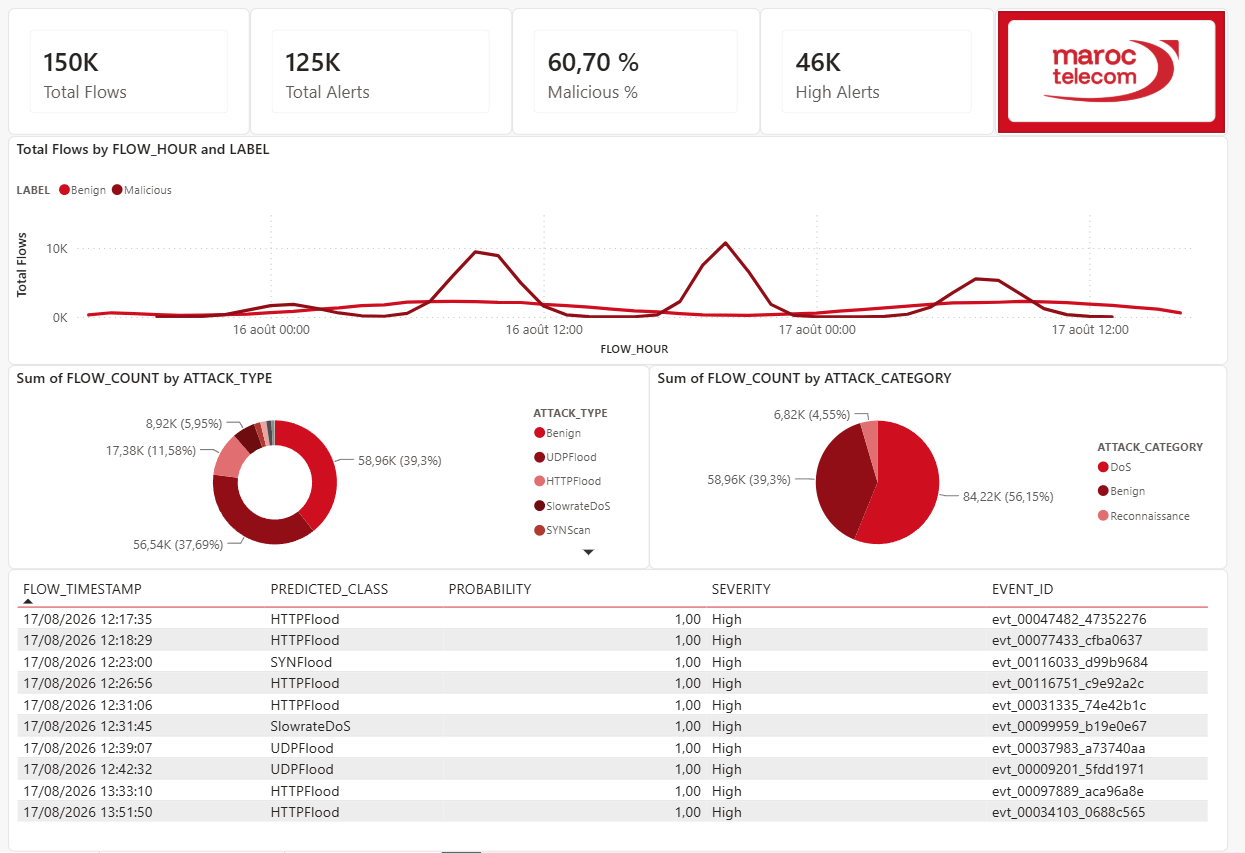
\includegraphics[width=\textwidth]{Page1-power-bi.png}
\caption{Page 1 : vue d'ensemble SOC, indicateurs clés, évolution du trafic et dernières alertes.}
\end{figure}

\subsection{Page 2 : Analyse des attaques}
Cette page approfondit la nature des menaces. Elle présente l'évolution des attaques par type, la comparaison entre attaques par saturation et reconnaissance dans le temps, la répartition par outil d'attaque, une matrice de chaleur croisant le protocole et le type d'attaque, ainsi qu'un tableau de profil précisant le débit, la durée et la volumétrie par attaque. La comparaison temporelle met en évidence une phase de reconnaissance précédant les vagues de saturation.

\begin{figure}[H]
\centering
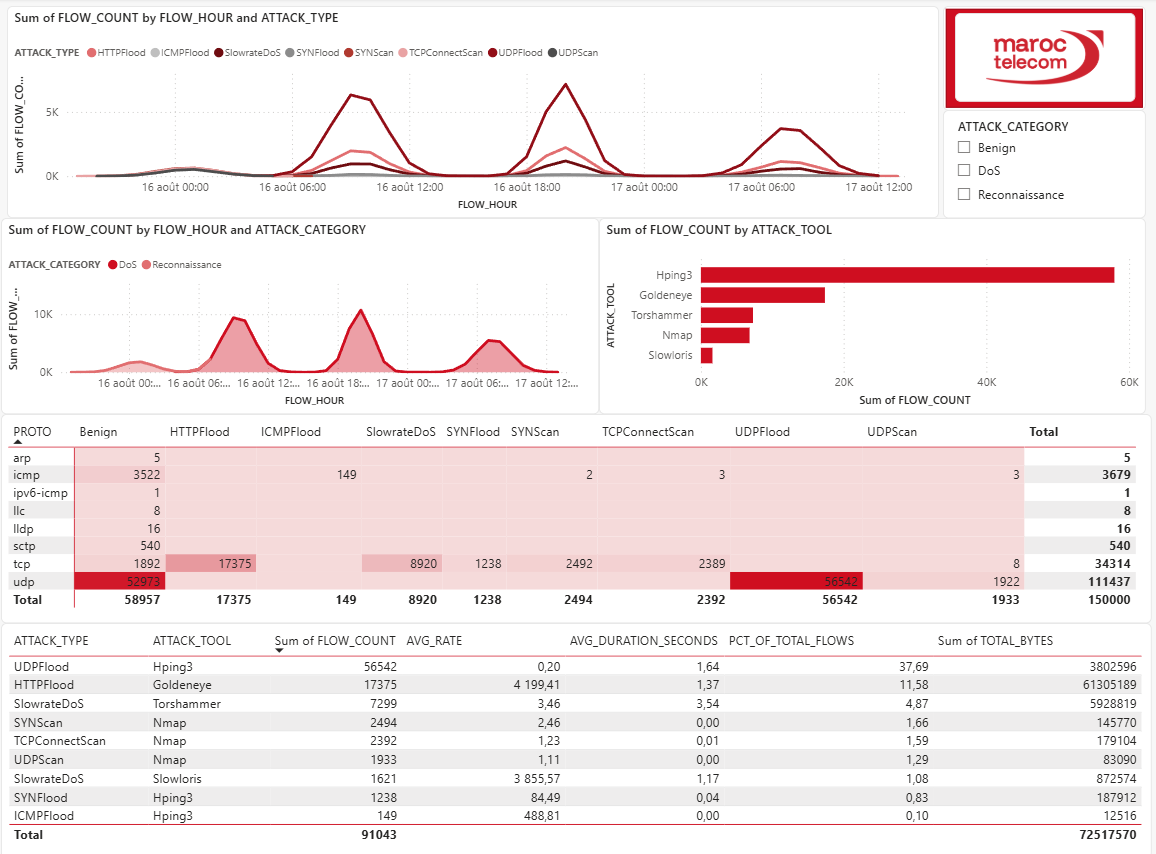
\includegraphics[width=\textwidth]{page2.png}
\caption{Page 2 : analyse des attaques, dynamique temporelle, matrice protocole par type et profils.}
\end{figure}

\subsection{Page 3 : Explicabilité et supervision}
Cette page rend le modèle transparent. Elle affiche l'importance globale des variables selon SHAP, les variables les plus déterminantes par type d'attaque au moyen d'un filtre interactif, ainsi qu'un bloc de suivi de dérive comprenant un verdict, un indice de dérive par variable et un tableau de détail. Elle répond à l'exigence de confiance en permettant de comprendre pourquoi un flux est classé comme une menace.

\begin{figure}[H]
\centering
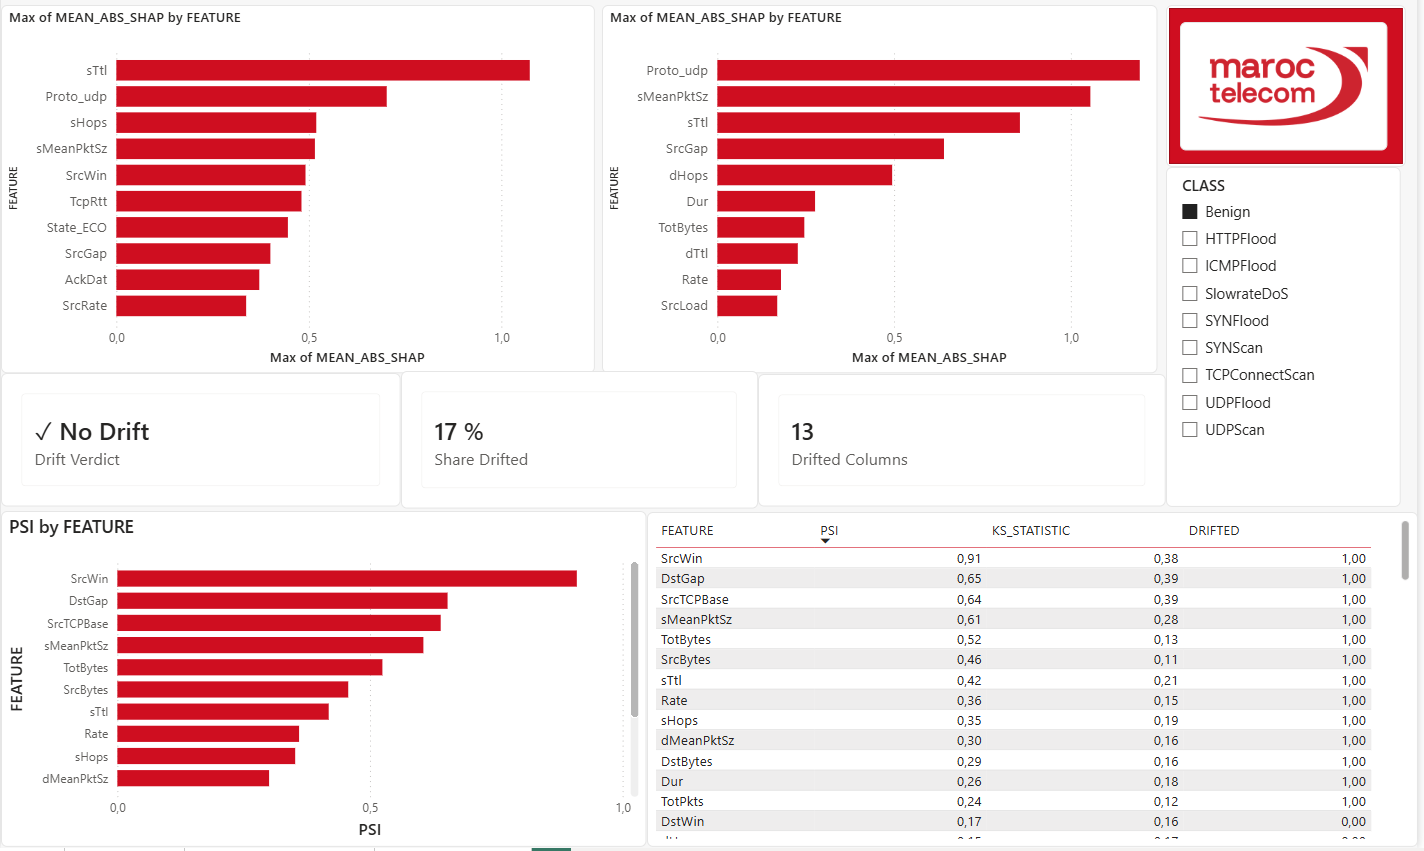
\includegraphics[width=\textwidth]{page3.png}
\caption{Page 3 : explicabilité par SHAP et supervision de la dérive des données.}
\end{figure}

\subsection{Page 4 : Modèle et qualité des données}
Cette page consolide la fiabilité de la chaîne. Elle regroupe des cartes de performance (version du modèle, exactitude, F1 macro), la précision et le rappel par classe, un tableau de métriques détaillées, ainsi que les indicateurs de qualité des données, à savoir le taux de validation, le nombre d'enregistrements contrôlés et le nombre de contrôles en échec.

\begin{figure}[H]
\centering
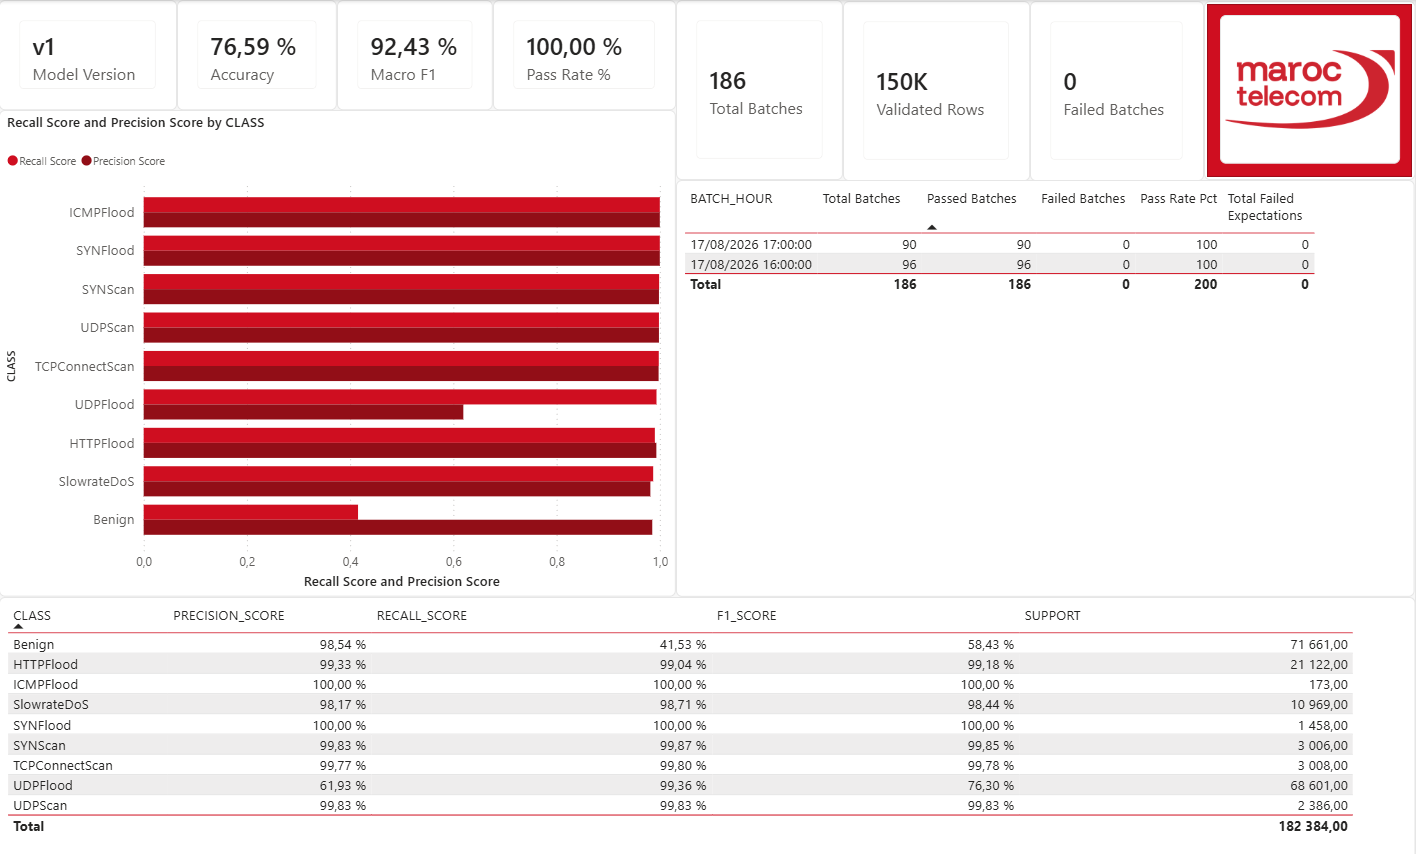
\includegraphics[width=\textwidth]{page4.png}
\caption{Page 4 : performance du modèle et qualité des données.}
\end{figure}

%=====================================================================
\chapter{Enrichissement par le Machine Learning et l'Explainable AI}

La couche décisionnelle décrite précédemment ne prend toute sa valeur que si les flux qu'elle restitue sont \textbf{correctement qualifiés}. Tel est le rôle de la couche d'enrichissement. Un modèle d'apprentissage automatique attribue à chaque flux une classe, bénigne ou correspondant à un type d'attaque, et une couche d'IA explicable justifie ses décisions. Cette couche est présentée ici en tant que source d'alimentation de la solution BI, et non comme finalité.

\section{Préparation des données et gestion du déséquilibre}
Les enregistrements de flux comportent des valeurs manquantes \emph{structurelles}. Par exemple, certains champs propres au protocole TCP sont absents pour les flux UDP ou ICMP. Plutôt qu'une imputation par la moyenne, une stratégie de \textbf{valeur sentinelle} accompagnée d'indicateurs booléens a été retenue, afin que le modèle distingue le cas « non applicable » du cas « applicable mais nul ». Les variables catégorielles ont été encodées en indicatrices.

Le jeu de données présente un fort \textbf{déséquilibre de classes}, la classe la plus rare ne représentant qu'une fraction de pourcent. La métrique de référence retenue est donc le \textbf{F1 macro}, qui pondère équitablement toutes les classes. Le déséquilibre a été traité par pondération des exemples à l'entraînement.

\section{Comparaison des modèles}
Trois familles de modèles ont été comparées sur un jeu de validation : la régression logistique, la forêt aléatoire et le gradient boosting (XGBoost).

\begin{table}[h]
\centering
\caption{Comparaison des modèles sur le jeu de validation}
\begin{tabularx}{\textwidth}{Xccc}
\toprule
\textbf{Métrique} & \textbf{Rég.\ logistique} & \textbf{Forêt aléatoire} & \textbf{XGBoost} \\
\midrule
Exactitude & 0,76 & 0,72 & 0,77 \\
F1 macro   & 0,91 & 0,92 & \textbf{0,92} \\
F1 pondéré & 0,74 & 0,72 & 0,75 \\
\bottomrule
\end{tabularx}
\end{table}

Les trois familles convergent vers un F1 macro voisin de 0,92. Ce résultat indique que la performance est \textbf{limitée par la représentation des données} plutôt que par la puissance du modèle. Le modèle \textbf{XGBoost} a été retenu comme modèle de production, pour son léger avantage et pour son excellente compatibilité avec l'explicabilité par SHAP.

\section{Modèle retenu et compromis opérationnel}
Évalué sur un jeu de test indépendant, le modèle atteint une \textbf{exactitude de 0,77} et un \textbf{F1 macro de 0,92}. Huit des neuf classes obtiennent une précision et un rappel compris entre 0,98 et 1,00. La seule difficulté réside dans une \textbf{confusion résiduelle} entre le trafic bénin à fort volume et une attaque par saturation UDP. Le modèle privilégie la détection exhaustive des attaques, avec un rappel proche de 1, au prix d'un sur-signalement de certains flux légitimes. Ce compromis est \textbf{favorable en contexte de sécurité}, car il vaut mieux vérifier une fausse alerte que manquer une attaque réelle.

\begin{figure}[h]
\centering
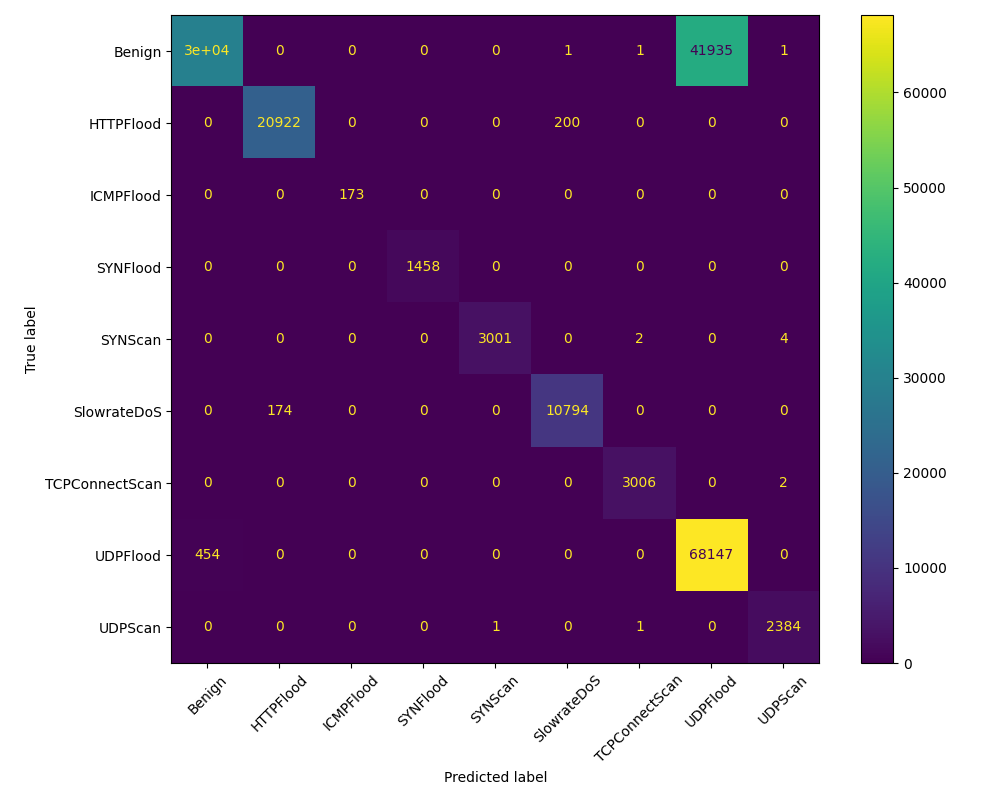
\includegraphics[width=0.82\textwidth]{confusion_matrix_prod.png}
\caption{Matrice de confusion du modèle retenu (classification multiclasse sur le jeu de test).}
\end{figure}

\section{Explicabilité par SHAP}
Pour instaurer la confiance des décideurs, les décisions du modèle sont rendues interprétables au moyen de la méthode \textbf{SHAP}. L'importance globale des variables et les contributions par classe sont calculées puis exportées sous forme de table interrogeable, directement exploitée par la page d'explicabilité de Power BI. Les variables les plus déterminantes relèvent de la signature réseau, à savoir le temps de vie, le protocole, le nombre de sauts et la taille moyenne de paquet, ce qui reste cohérent avec la nature des attaques observées.

\begin{figure}[h]
\centering
\includegraphics[width=0.82\textwidth]{modeling/artifacts/shap/shap_global_bar.png}
\caption{Importance globale des variables selon SHAP.}
\end{figure}

\begin{figure}[h]
\centering
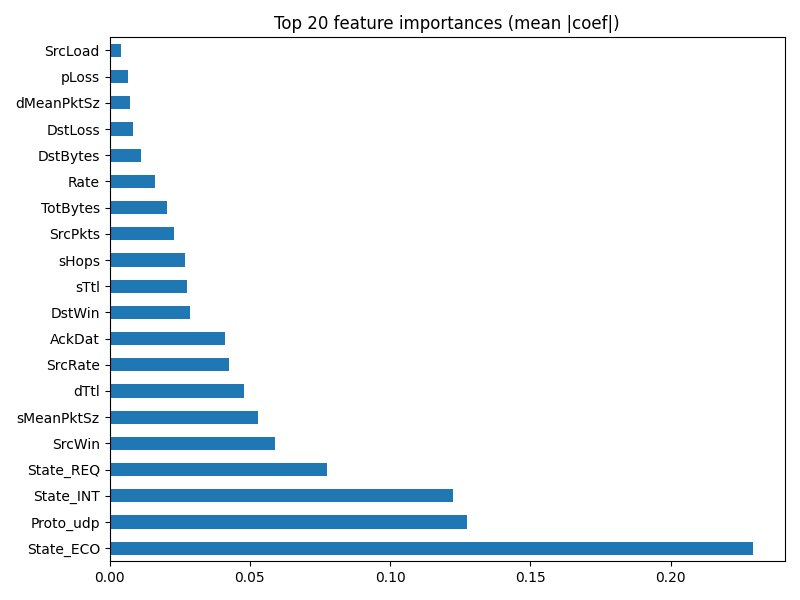
\includegraphics[width=0.82\textwidth]{feature_importance_prod.png}
\caption{Importance des variables selon le gain du modèle, vue complémentaire.}
\end{figure}

%=====================================================================
\chapter{Intégration globale, industrialisation et suivi}

\section{Architecture d'ensemble}
La solution s'inscrit dans une architecture en couches, dite médaillon, qui achemine la donnée de la source jusqu'à la restitution :

\begin{enumerate}[leftmargin=1.6em]
  \item \textbf{Ingestion en flux.} Un simulateur rejoue les enregistrements de flux vers un bus de messages, reproduisant un flux temps réel.
  \item \textbf{Traitement distribué.} Des traitements Apache Spark en continu constituent une couche Bronze, contenant les données brutes, puis une couche Argent, contenant les données typées et nettoyées, stockées sur un système objet compatible S3.
  \item \textbf{Contrôle qualité.} Chaque micro-lot est validé par Great Expectations, dont les résultats alimentent un indicateur de qualité.
  \item \textbf{Enrichissement.} Un service de scoring applique le modèle et produit la couche Or, composée des prédictions et des alertes.
  \item \textbf{Entreposage et modélisation.} Les tables Or sont chargées dans Snowflake, où dbt construit les tables décisionnelles.
  \item \textbf{Restitution.} Power BI se connecte aux tables Or et expose les tableaux de bord.
\end{enumerate}

\section{Service du modèle et gestion du cycle de vie}
Le modèle est exposé au reste de la chaîne par une \textbf{interface applicative} développée avec FastAPI. Cette interface applique en interne l'ensemble des transformations d'entraînement, à savoir l'encodage, le calcul des indicateurs et l'alignement des variables, afin de garantir une source unique de vérité pour la préparation. Le cycle de vie du modèle, comprenant les versions, les alias de promotion et les artefacts, est géré par \textbf{MLflow}. Ce dispositif permet de faire évoluer le modèle sans reconstruire la chaîne.

\section{Suivi de la dérive des données}
La pérennité d'un modèle en production dépend de la stabilité des données qu'il reçoit. Un dispositif de \textbf{suivi de dérive} compare la distribution des flux courants à une distribution de référence, au moyen de l'indice PSI et d'un test statistique. Le verdict global et les indices par variable sont exportés vers la couche Or et restitués dans Power BI. Les responsables disposent ainsi d'un indicateur d'alerte précoce en cas de dérive significative.

\section{Processus d'actualisation}
L'actualisation de la solution suit un processus reproductible : régénération de la couche Or, rechargement des tables dans Snowflake, reconstruction des tables décisionnelles dbt, puis rafraîchissement du modèle Power BI. Ce séquencement garantit la cohérence entre les indicateurs affichés et l'état réel des données.

%=====================================================================
\chapter*{Conclusion et perspectives}
\addcontentsline{toc}{chapter}{Conclusion et perspectives}

Ce projet a permis de concevoir et de réaliser une \textbf{solution décisionnelle complète sous Power BI} pour la supervision de la sécurité des réseaux 5G, en cohérence avec la logique de pilotage propre au pôle Contrôle de Gestion de Maroc Telecom. Le livrable central est un tableau de bord de type SOC composé de quatre pages et habillé aux couleurs de l'entreprise. Il restitue de manière lisible et interactive l'activité du réseau, la nature des menaces, l'explicabilité des détections et la fiabilité de la chaîne.

La valeur de la solution tient à sa \textbf{cohérence de bout en bout}. Elle repose sur un modèle de données organisé et performant, sur des indicateurs centralisés, sur une préparation maîtrisée via Power Query, ainsi que sur une alimentation par des couches d'enrichissement et d'ingénierie de données industrialisées. L'accent mis sur la transparence, sur la qualité et sur le suivi de la dérive confère à la solution la crédibilité attendue d'un outil de contrôle de gestion.

Plusieurs \textbf{perspectives d'évolution} se dessinent. Sur le plan décisionnel, il serait pertinent d'ajouter un axe de restitution par alerte offrant une explication individuelle, d'historiser les performances par version de modèle et de suivre la dérive dans le temps. Sur le plan de l'industrialisation, la conteneurisation complète des services, déjà amorcée avec Docker, pourrait être poursuivie par leur orchestration à l'échelle avec Kubernetes et par l'automatisation des traitements périodiques avec Airflow. Enfin, le branchement de la chaîne sur des flux réellement temps réel constituerait l'étape naturelle vers une exploitation opérationnelle.

Au-delà du livrable, ce stage aura été l'occasion d'appréhender concrètement l'ensemble de la chaîne de valeur de la donnée, de l'ingénierie jusqu'à la décision, et de mesurer combien la restitution décisionnelle constitue le maillon qui transforme une capacité technique en véritable outil de pilotage.

%=====================================================================
\begin{thebibliography}{9}
\addcontentsline{toc}{chapter}{Bibliographie}
\bibitem{powerbi} Microsoft, \emph{Documentation Power BI}, learn.microsoft.com/power-bi.
\bibitem{dax} Microsoft, \emph{Référence du langage DAX}, learn.microsoft.com/dax.
\bibitem{kimball} R.\ Kimball, M.\ Ross, \emph{The Data Warehouse Toolkit}, Wiley.
\bibitem{shap} S.\ Lundberg, S.-I.\ Lee, \emph{A Unified Approach to Interpreting Model Predictions}, NeurIPS, 2017.
\bibitem{xgboost} T.\ Chen, C.\ Guestrin, \emph{XGBoost: A Scalable Tree Boosting System}, KDD, 2016.
\bibitem{grinsztajn} L.\ Grinsztajn et al., \emph{Why do tree-based models still outperform deep learning on tabular data?}, NeurIPS, 2022.
\bibitem{snowflake} Snowflake Inc., \emph{Snowflake Documentation}, docs.snowflake.com.
\bibitem{dbt} dbt Labs, \emph{dbt Documentation}, docs.getdbt.com.
\end{thebibliography}

%=====================================================================
\appendix
\chapter{Annexes}

\section*{A. Glossaire}
\begin{tabularx}{\textwidth}{lX}
\toprule
\textbf{Terme} & \textbf{Définition} \\
\midrule
Mesure DAX & Calcul d'indicateur évalué dynamiquement selon le contexte du visuel. \\
Couche Or & Niveau final, agrégé et prêt à l'analyse, d'une architecture médaillon. \\
SHAP & Méthode d'attribution de la contribution de chaque variable à une prédiction. \\
PSI & Indice mesurant l'écart entre deux distributions, utilisé pour le suivi de dérive. \\
Segment & Filtre visuel permettant de restreindre l'ensemble d'une page. \\
\bottomrule
\end{tabularx}

\section*{B. Organisation des travaux}
Le projet s'est organisé autour de couches complémentaires. Une couche de contrat de données a fixé la définition commune des variables. Une couche d'ingestion a assuré l'acheminement des flux. Une couche de traitement a construit les niveaux Bronze et Argent et a contrôlé leur qualité. Une couche de service a produit les prédictions et les alertes de la couche Or. Une couche de modélisation a pris en charge la préparation, l'entraînement, l'explicabilité et les exports. Une couche d'entreposage a rassemblé les chargements Snowflake et les tables décisionnelles. Enfin, une couche de restitution a porté le thème graphique et les tableaux de bord Power BI.

\section*{C. Principe d'échange avec le service de scoring}
Le service de scoring reçoit un ensemble de flux décrits par leurs caractéristiques brutes, accompagnés d'un identifiant d'événement. Il renvoie, pour chaque flux, la classe prédite, la probabilité associée et la version du modèle ayant produit la décision. Cet identifiant d'événement permet ensuite de rattacher chaque prédiction au flux correspondant lors de la construction de la couche Or.

\end{document}
